% !TEX root = SCPROG.tex
% This work is licensed under the Creative Commons
% Attribution-NonCommercial-ShareAlike 4.0 International License. To view a copy
% of this license, visit http://creativecommons.org/licenses/by-nc-sa/4.0/ or
% send a letter to Creative Commons, PO Box 1866, Mountain View, CA 94042, USA.

\tikzset{every picture/.style={line width=0.75pt}} %set default line width to 0.75pt        

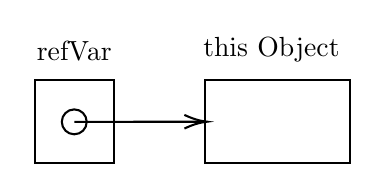
\begin{tikzpicture}[x=0.75pt,y=0.75pt,yscale=-1,xscale=1]
%uncomment if require: \path (0,300); %set diagram left start at 0, and has height of 300

%Shape: Rectangle [id:dp4673267372054163] 
\draw   (100,116) -- (138,116) -- (138,156) -- (100,156) -- cycle ;
%Shape: Rectangle [id:dp7209025887395226] 
\draw   (182,116) -- (252,116) -- (252,156) -- (182,156) -- cycle ;
%Shape: Circle [id:dp9831972127744683] 
\draw   (113,136) .. controls (113,132.69) and (115.69,130) .. (119,130) .. controls (122.31,130) and (125,132.69) .. (125,136) .. controls (125,139.31) and (122.31,142) .. (119,142) .. controls (115.69,142) and (113,139.31) .. (113,136) -- cycle ;
%Straight Lines [id:da3061374812316927] 
\draw    (119,136) -- (181,135.94) ;
\draw [shift={(183,135.93)}, rotate = 539.94] [color={rgb, 255:red, 0; green, 0; blue, 0 }  ][line width=0.75]    (10.93,-3.29) .. controls (6.95,-1.4) and (3.31,-0.3) .. (0,0) .. controls (3.31,0.3) and (6.95,1.4) .. (10.93,3.29)   ;


% Text Node
\draw (119,102) node  [align=left] {refVar};
% Text Node
\draw (214,101) node  [align=left] {this Object};


\end{tikzpicture}
